%%
%% This is file `mcmthesis-demo.tex',
%% generated with the docstrip utility.
%%
%% The original source files were:
%%
%% mcmthesis.dtx  (with options: `demo')
%%
%% -----------------------------------
%%
%% This is a generated file.
%%
%% Copyright (C)
%%     2010 -- 2015 by Zhaoli
%%     2014 -- 2016 by Liam 
%%     2017 -- 2019 by Xuehan
%%
%% This work may be distributed and/or modified under the
%% conditions of the LaTeX Project Public License, either version 1.3
%% of this license or (at your option) any later version.
%%
%% This work has the LPPL maintenance status `maintained'.
%%
%% The Current Maintainer of this work is Xuehan.
%%
\documentclass{mcmthesis}
\bibliographystyle{IEEEtran}
\mcmsetup{CTeX = false,   % 使用 CTeX 套装时,设置为 true
        tcn = 2002134, problem = D,
        sheet = true, titleinsheet = true, keywordsinsheet = true,
        titlepage = true}
\usepackage{palatino}
\usepackage{mwe}
\usepackage{graphicx}
\usepackage{subcaption}
\usepackage{float}
\usepackage{multirow}
\usepackage{indentfirst}
\usepackage{gensymb}
\usepackage[ruled,lined,commentsnumbered]{algorithm2e}
\usepackage{geometry}


\begin{document}
\linespread{0.6} %%行间距
\setlength{\parskip}{0.5\baselineskip} %%段间距
\title{ti}

\date{\today}
	\begin{abstract}

	
		\begin{keywords}
		
		\end{keywords}
	\end{abstract}

\maketitle

\tableofcontents

\newpage

\section{Introduction}
\subsection{Problem Background}
	Football is one of the most well-known sports activities in the world.  The standard system of an 11-man football game is one goalkeeper and 10 players from each of the two teams. There are a total of 22 players who fight, defend and attack on the rectangular grass court.  The game scores by shooting the ball into the opponent's goal. When the game is over, the team with the most points wins.

	\begin{figure}[h]
		\centering
		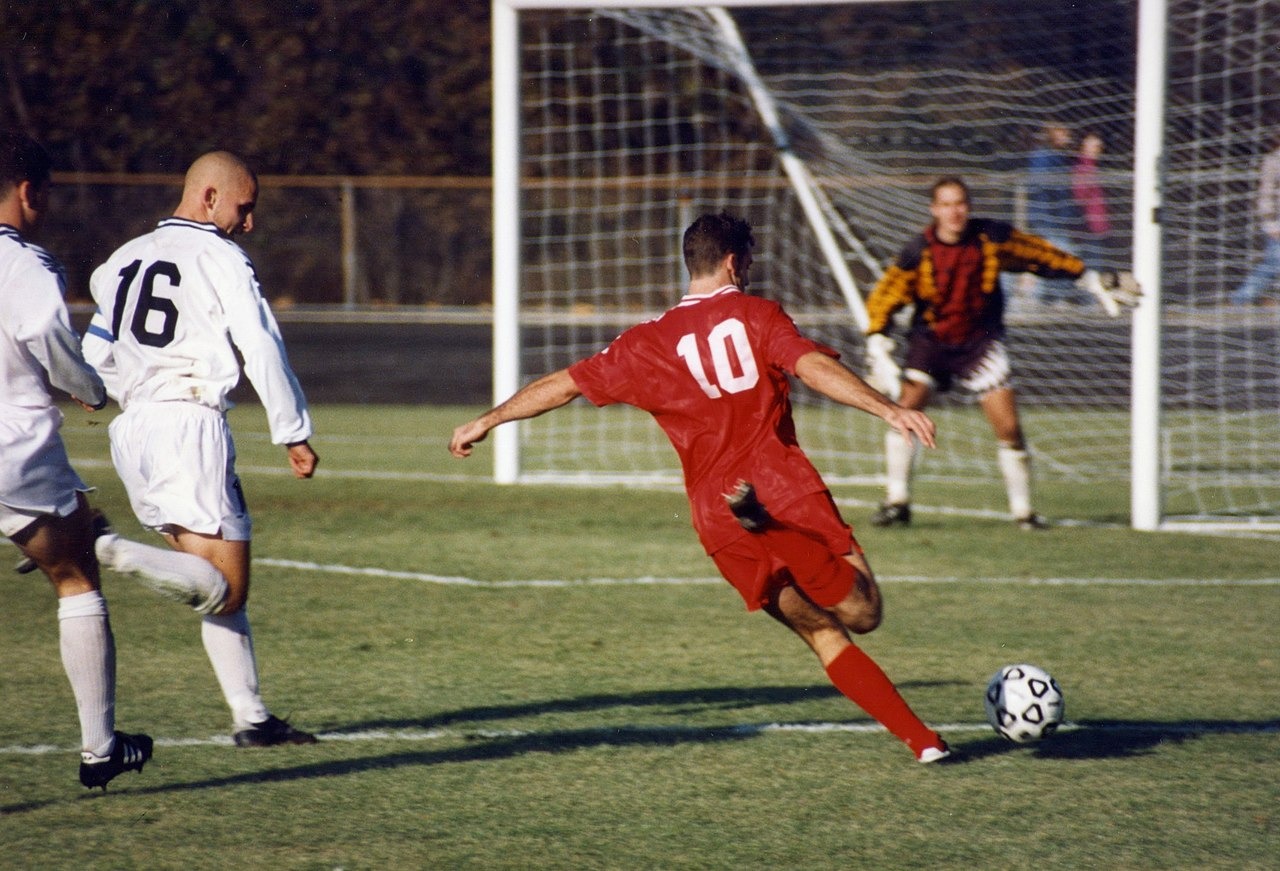
\includegraphics[width=0.75\textwidth]{figures/football.jpg}
		\caption{A Football Game~\cite{Wiki_Football}}
	\end{figure}

	As we all know, football is a sport that requires intense teamwork.  For it can show the importance of teamwork spirit more than superb personal ability.  Passing, as an offensive means that requires the cooperation of various players to play the biggest role, is just an important manifestation of the team spirit of football.  Therefore, to study the important role of teamwork in football, you can start by studying the passing network in football.

	Our goal is to build a network model to simulate the Huskies' passing network and study it.  Meanwhile, it is necessary to extract some representative parameters from the constructed network model.  Through the study of such parameters, we can accurately understand the team collaboration ability and structural characteristics of this team.
\subsection{Our Work}
	In this paper, we successfully built the Huskies' passing network model.  On the basis of this network model, we obtained some important parameters. In this way, we analyzed the team collaboration ability of the Huskies players, and offered some suggestion for its future structural strategy.

	In Section 2, we state some basic assumptions.  Section 3 contains the nomenclature used in the statement of our model.  Section 4 provides sufficient details about our network model.  Section 5 carries on the simulation experiment and analysis to our proposed model.  Section 6 provides some advice on its structural strategies for the Huskies.  Finally, we further analyze the sensitivity, advantages and disadvantages of our model in Section 7, and we obtain some conclusions on how to improve the teamwork spirit of general teams in Section 8.
\section{Assumptions}
	Our model is based on these following basic assumptions:
	\begin{enumerate}
		\item The average position of a player over a period of time is equivalent to the average of the position of the player in all events that occurred during that period.
	\end{enumerate}
\section{Nomenclature}
	Symbols that our model mainly uses are listed in Table \ref{tab:Nomen}.  Other symbols that are used only once will be described in the following chapters.
	\begin{table}
    	\centering
    	\caption{Nomenclature}
		\label{tab:Nomen}
		\begin{tabular}{c c}
			\hline
					Symbol & Definition\\
			\hline
				$\textbf{A}$ & Football passing matrix\\
				$\textbf{B}$ & Adjacency matrix\\
				$a_{i}$ & The \emph{i}th player in Huskies\\
				$a_{ij}$ & Number of passes from player $i$ to player $j$\\
				$\langle$$X$$\rangle$ & The x-coordinate of the network centroid\\
				$\langle$$Y$$\rangle$ & The y-coordinate of the network centroid\\
				$D$ & The dispersion of the position of the players around the network centroid\\
			\hline
   	 	\end{tabular}
	\end{table}

\section{The Basic Model}
	In this section we will discuss our network model in detail.  First of all, we will begin with the establishment of our network model.  Then we will use our model to identify some patterns of the network.  Finally, we will also investigate the indicators of teamwork. 
\subsection{Build of the Network}

\subsection{Identify Network Patterns}
\subsection{Identify Teamwork Indicators}
\section{Implementation}
\section{Structural Strategies}
\section{Model Analysis}
\subsection{Sensitivity Analysis}
\subsection{Strengths and Weakness}
\section{Conclusion}

\bibliography{ref}
\newpage

\begin{appendices}


\end{appendices}

\end{document}
